
\subsection{Generalized Graph Grammars $\mathcal{G}$ for Nested Graphs. $\qtransl_{\mathcal{H},\mathcal{T}}^{\mathcal{G}}(\mathcal{H})(\nested)$}\label{subsec:gggSec}\label{sec:semistructunstradata}
%%%%%%%%%%%%%%%%%%%%%%%%
%%%%%%%%%%%%%%%%%%%%%%%%
%%%%%%%%%%%%%%%%%%%%%%%%
%%%%%%%%%%%%%%%%%%%%%%%%
%\subsection{(*) Semi-structuring unstructured data}
We continue to both analyse the dependency graph semistructured representation for unstructured data (as already introduced in Section \vref{sec:idifud}), and search for a $\Qoppa$ definition. As also remarked in Section \vref{sec:unstructured}, the problem with representing unstructured data is that they lack of a precise data structure that could be directly queried, handled and created by automated processes. As a consequence, some ``structure'' has to be provided.



%In those other use cases, different techniques are used: %can be only used as an intermediate representation for relation extraction processes, because it does not provide useful information to be extracted as the relations showed as desired result in both IBM Watson and DeepDive's  \textbf{Knowledge Base Construction} phase . 
%\begin{example}[label=ex:introgrammars]
	%Figure \ref{fig:dependencygraph} provides an example of a dependency graph  directly generated from full-text using Stanford NLP library. In particular, the full text is represented as a graph, where each word is represented in its flexed form as a vertex (\textit{entity}). Edges (\textit{relationships}) correspond to \textbf{universal dependencies}\footnote{\url{http://universaldependencies.org}} \cite{MarneffeDSHGNM14}, which are grammatical functions connecting different parts of speech. 
	If we suppose that the full text is well written and that it follows the correct grammar rules of its natural language, then we can express such full text as a dependency graph (Figure \vref{fig:dependencygraph}), and we can express grammatical rules through graph grammar operations. In particular, we can use graph pattern matching queries to match all the foreseeable natural language's constructs, and then transform them into a nested graph, where entities will represent whole \textit{complements} or whole sentences (e.g., \textit{dependent or subordinate clauses}), and verbs - representing actions from the subject to the object or from the agent towards the subject - represent edges connecting the former concepts through linguistic relationships. 
	

\begin{figure*}[!p]
	\centering
	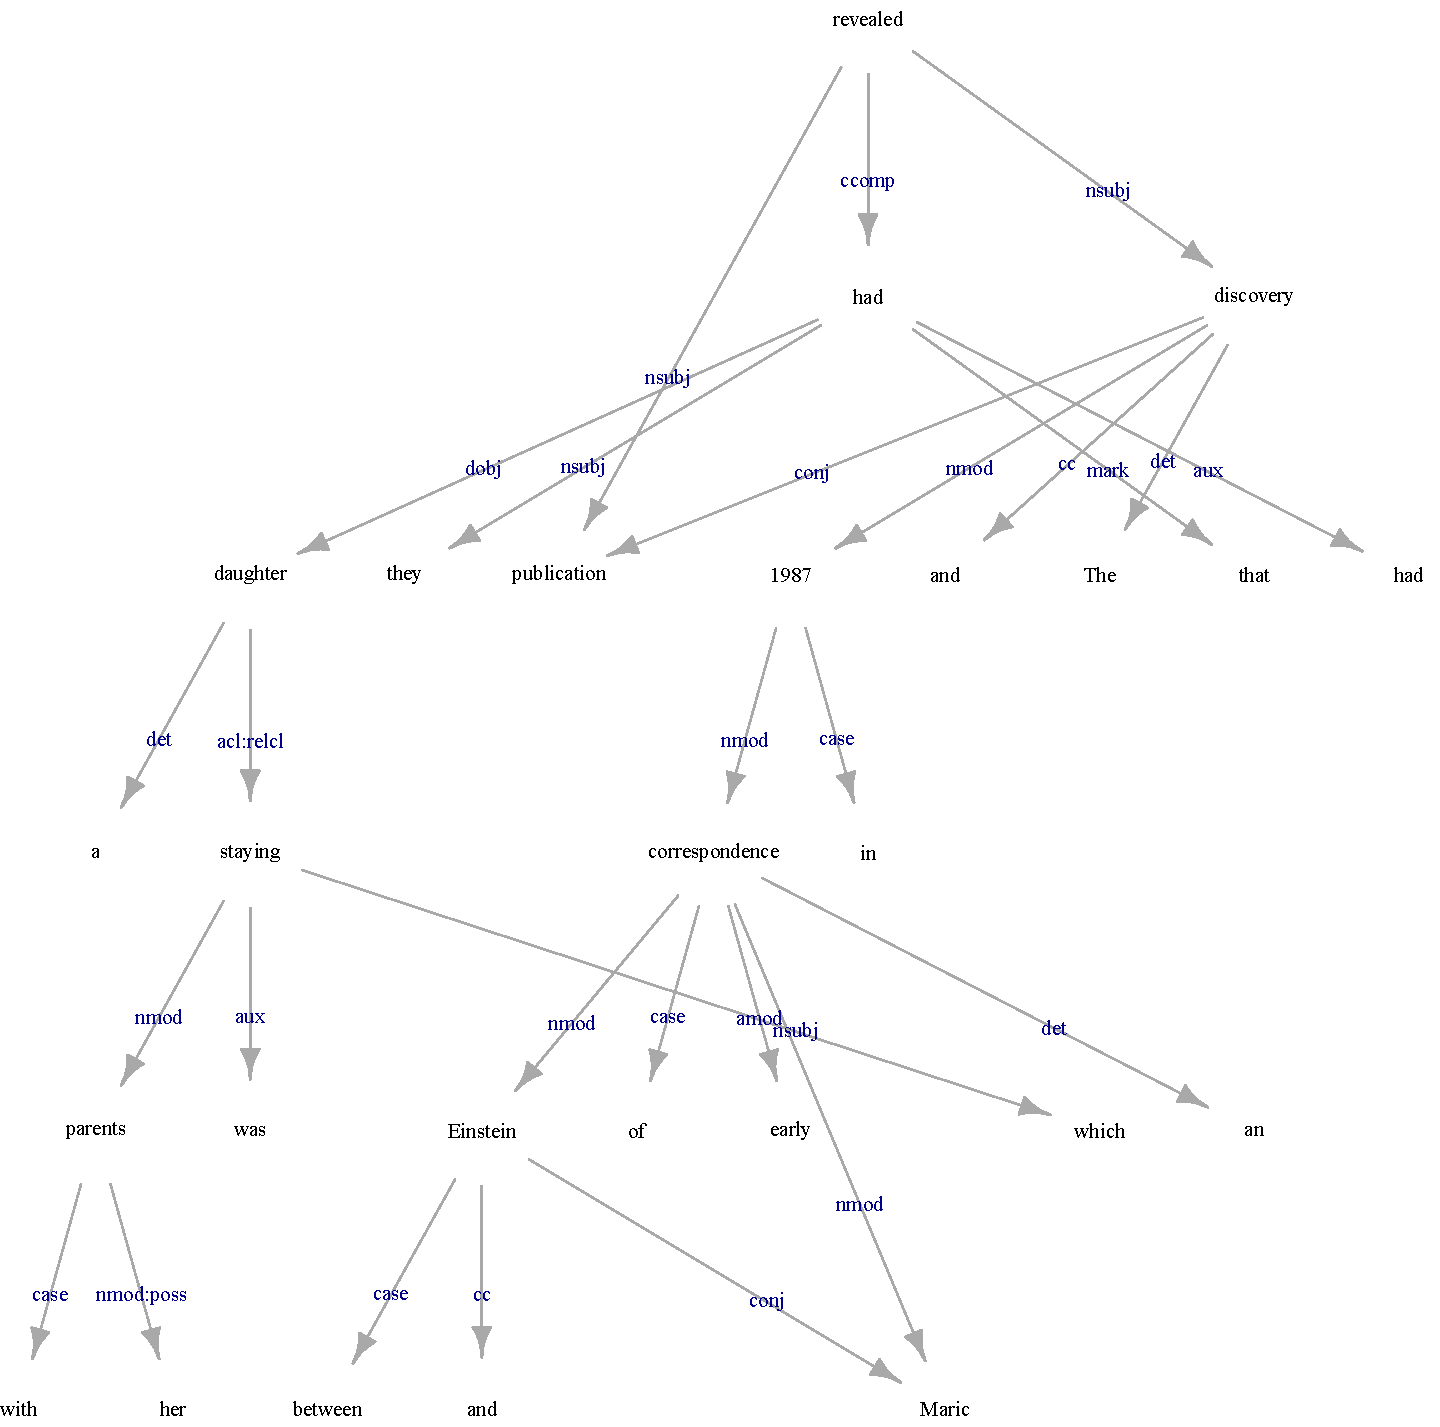
\includegraphics[width=\textwidth]{fig/05language/00DependencyGraph}
	\caption{Graph representation of the following sentence from Wikipedia: ``\textit{The discovery and publication in 1987 of an early correspondence between Einstein and Maric revealed that they had had a daughter was staying with her parents.}''. }
	\label{fig:dependencygraph}
\end{figure*} 
\begin{figure*}[!pth]
	\begin{minipage}[b]{\textwidth}
		\centering
		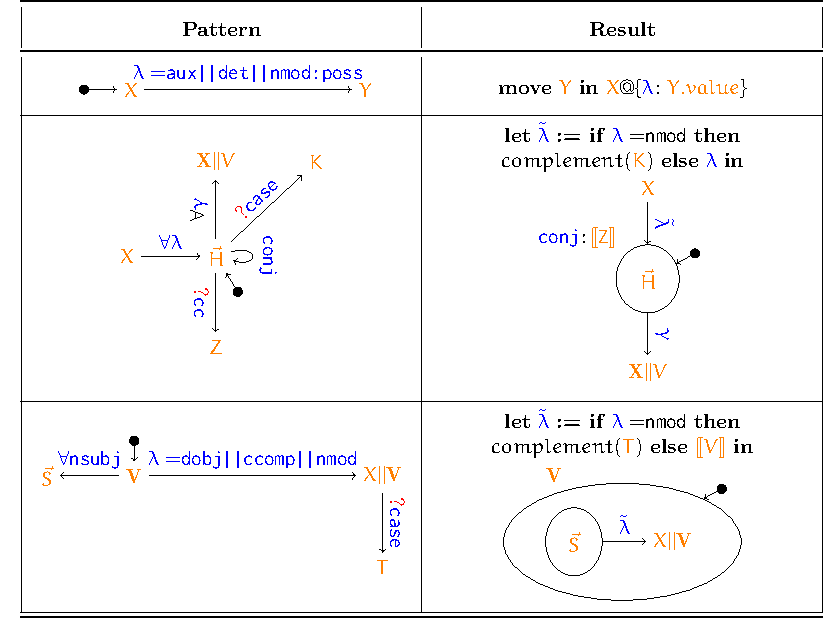
\includegraphics[width=\textwidth]{fig/05language/diagramtable}
		\subcaption{Query for nested graph allowing to rewrite the full-text graph representation.}
		\label{fig:diagramtable}
	\end{minipage}
	\begin{minipage}[b]{\textwidth}
		\centering
		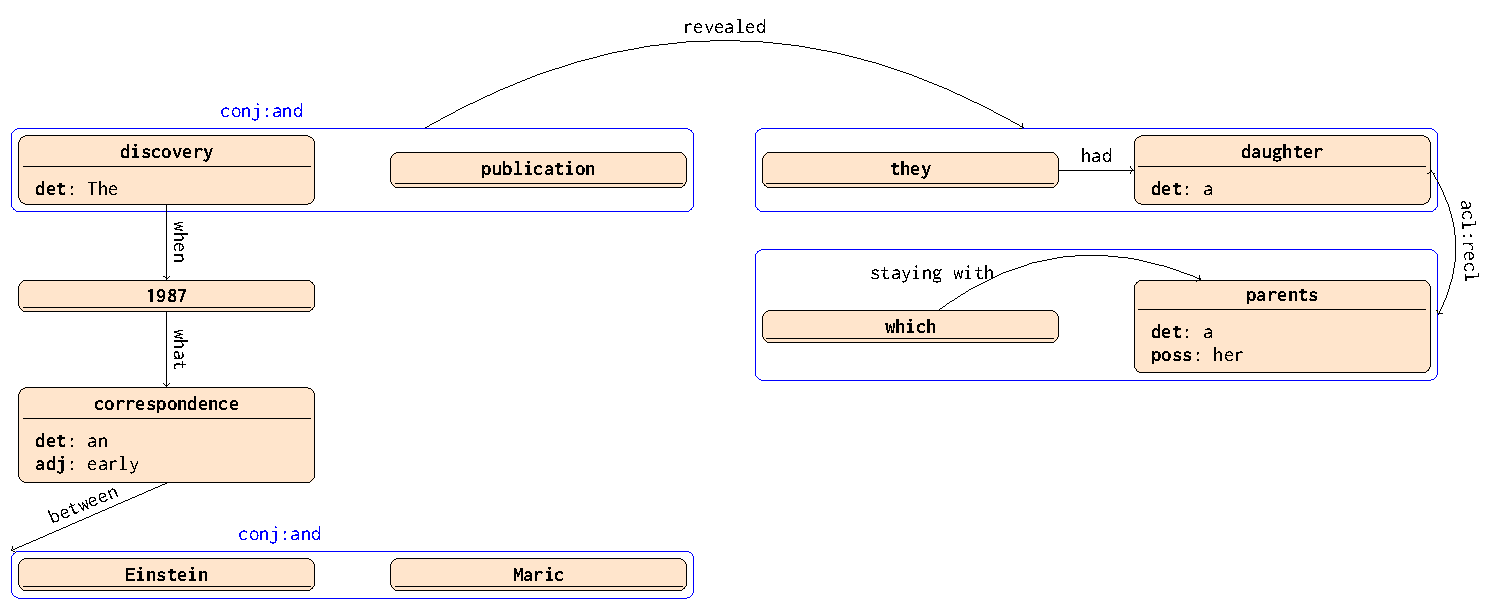
\includegraphics[width=1.2\textwidth]{fig/05language/nestedrepr}
		\subcaption{Result of the application of the patterns in Figure \subref{fig:diagramtable}.}
		\label{fig:nestedrepr}
	\end{minipage}
	\caption{Translating the full-text representation as a graph in Figure \ref{fig:dependencygraph}: this requires a graph transformation language and the definition of nested graphs.}
	\label{fig:globalconversiontext}
\end{figure*}
	On the footsteps of GraphLOG, Figure \ref{fig:diagramtable} represent an example of a visual representation of match and rewrite rules: we want to match the graphs represented in the ``pattern'' column, and rewrite them as the nested graphs presented within the ``result'' column. 
	The first rule tells that each vertex $\color{orange}X$ that has outgoing edges with one of the labels depicted in $\color{blue}\lambda$ has to be updated with the $\color{orange} value$ stored in its correspondent adjacent vertex $\color{orange} Y$. The second rule tells to collect inside one single nested vertex all the elements that are in conjunction $\color{blue}conj$ with each other through a conjunction $\color{orange} Z$: moreover, any other ingoing and outgoing edge to this nested object of a given label  must be rewritten as a single ingoing or outgoing edge. The last one tells to rewrite the verb of a sentence, represented as a root $\color{orange} V$ linked to the list of subjects $\color{orange} \vec{S}$ and the object $\color{orange}X||V$ (that can be a verb being a root of another sentence), as a whole nested vertex containing an edge to the nested object of all the components of the subject, directed to the final object or sentence. 
	In particular,  graph grammars are defined through the combination of such rewriting rules   \cite{GraphLogAggr,Plump1998Term}: the former  picture also shows how such match and rewrite query can be expressed by a visual formalism, instead of being coded using a specific programming language as already showed in the early 90s \cite{GraphLogAggr}.
	
	
	A possible outcome of such pattern matching and transformation is provided in Figure \ref{fig:nestedrepr}: this  result is both more human readable and machine readable than the first sentence input, thus allowing a computer to better analyse the content of the sentence. As we have already seen in Section \vref{subsec:ggram}, graph grammars neither allow to nest graphs nor allow to fully transform the matched vertices and edges. Consequently, a generalization of such approach is required, also permitting one single rewriting graph (hub schema) towards which multiple matching graph can be transformed to. The following definition provides us a preliminary and wordy definition, that is going to be formalized after an exaplainatory running example on a much simpler use case involving bibliography graphs. 
	
	 %In particular, 
	
	
	% An example of how such analysis is possible will be provided in one of the next examples (more precisely, Example \vref{ex:nestalign}).
%\end{example}






%As a first step, we want to generalize the concept of graph grammars, in order to make them a suitable replacement of the application of several graph pattern (or graph traversal) matching problems, and to be able to transform nested graphs. For this reason, generalized graph grammars shall be defined as a nested graph operator as follows, in the following preliminary definition:

\begin{definition}[Generalized Graph Grammars]\label{def:gggintro}
A \textbf{generalized graph grammar}\footnote{See Sherlock for both a representation of nested graphs and an implementation of such generalized graph grammars: \url{https://bitbucket.org/unibogb/sherlock}}\index{graph grammar!generalized|textbf} is a collection of $n$ graph rewriting rules $[H_i\to T_i]_{i\leq n}^{m^i}$ applied to nested graph $\nested$ via the following operator $\mathcal{G}^{m_1,\dots,m_n}_{[H_i\to T_i]_{i\leq n}}(\nested)$, returning another nested graph. In particular, the set of all the $H_i$s appearing in the rules is denoted by $\mathcal{H}$, while the $T_i$s are referenced by $\mathcal{T}$.

The associated semantics of such graph grammar on a given nested graph in input $\nested$ is the following: each graph head $H_i$ provides a graph query which is going to be interpreted through a semantics $m^i$ returning a collection $m^i_{H_i}(N)$ of morphisms $f_j$ as a result of the matching phase. 

The associated transformation $T_i$ is described through a nested graph, and it is instantiated on each generated morphism $f_j$ generating several graphs replacing the matched ones. Each transformation graph $T_i$ may contain \begin{mylist}
\item \label{iitem} vertices (and/or edges) $o_h$ also contained\footnote{We preferred to use object identity instead of using further morphisms as in both graph grammars and nested graph alignments' refinement as in the previous chapter. Transformations and embeddings are going to be expressed as target objects' containments.} in $H_i$  providing the semantics ``return all the matched vertices (and/or edges) by a given vertex (and/or predicate) represented by $o_h$'' and possibly apply a transformation,
\item \label{iiitem} or new vertices (and/or edges) $o_c$ that are not in the vertex set $\phi(\ngraph,\ONTA)$, thus providing the semantics ``transform (or aggregate) the matched vertices (and/or edges) according to the (aggregation) functions of $o_c$''. Consequently,
\item \label{iiiitem} all the vertices (and edges) that are matched in $H_i$ but not returned as vertices in \ref{iitem}  (or  edges linking vertices that are neither contained in other objects nor appear as vertices in the final result) are removed from the returned graph.
	\end{mylist} In particular, all the edges generated in \ref{iiitem} must be associated with all the returned or generated vertices by the pattern.
\end{definition}

For the moment, we provide a wordy definition of such operator. The following example provides an explanation of such graph operator and is going to motivate the operator's subsequent formalization.


\begin{example}[label=ex:firstforgrammars]
	With reference to Example \vref{ex:bigraphbibnet}, we want to show how such aggregation is possible by simply using graph grammar rules.	In order to obtain the same result in Figure \vref{fig:aggrbibex}, we can use the Generalized Graph Grammars with just one rule $\mathcal{G}=[H\to T]^s$, where $H$ is the query ``return all the authors that are co-authors'' nested graph:
	\[H=(h,\Set{h,u_0,u_1,p_0,e_0,e_1},\ell,\xi,\phi)\]
	\[\ell(u_0)=\Set{\texttt{Author}}=\ell(u_1)\qquad \ell(p_0)=\Set{\texttt{Paper}}\qquad \ell(e_1)=\Set{\texttt{AuthorOf}}=\ell(e_2)\]
	\[\xi(u_0)=[\mstr{isGroupBy},\textup{\color{webgreen}``}\texttt{o.id != }u_1\textup{\color{webgreen}''}]\]
	\[\xi(u_1)=[\mstr{isGroupBy},\textup{\color{webgreen}``}\texttt{o.id != }u_0\textup{\color{webgreen}''}]\]
	\[\phi(h,\ONTA)=[u_0, u_1, p_0]\qquad \phi(h,\RELA)=[e_0, e_1]\]
	\[\phi(e_0,\SRC)=[u_0]\quad \phi(e_0,\DST)=[p_0]\quad \phi(e_1,\SRC)=[u_1]\quad \phi(e_1,\DST)=[p_0]\]
	This query then expresses that the pattern matching query must return the pattern fixing the two user (\mstr{isGroupBy}), and let return all the papers in common, and not just one single paper. We can enforce the fact that $u_0$ and $u_1$ cannot be the same user within the graph, if we allow vertices to insert predicates within their expressions as the second condition provided above.
	
	 The $T$ graph then must express that only the authors must be returned, a new edge between the co-authors must be created, and all the papers must be removed from the final result. In particular, the edge can contain all the papers that will be matched by $p_0$ as follows:
	\[(t,\Set{t,u_0,u_1,ca_0,p_0},\ell,\xi,\phi)\]
	\[\xi(ca_0)=[{\color{webgreen}\textup{``}\texttt{o.src!= o.dst}\textup{''}}]\]
	\[\ell(u_0)=\Set{\texttt{Author}}=\ell(u_1)\qquad \ell(ca_0)=\Set{\texttt{coauthorship}}\]
	\[\phi(t,\ONTA)=[u_0,u_1]\quad \phi(t,\RELA)=[ca_0]\]
	\[\phi(ca_0,\SRC)=[u_0]\quad \phi(ca_0,\DST)=[u_1]\quad \phi(ca_0,\mstr{pp})=[p_0]\]
	%\[\lambda(ca_0)=(u_0,u_1)\qquad ca_0(\texttt{pp})=(\cdot,[p_0])\]
	
	Since the grammar rules can only tell how to transform the matched subgraphs, we must first restrict the bibliography network $BN$ in Figure \vref{fig:inputbibex} into the greatest subgraph matching $H$: therefore, we're going to apply our graph grammar rules over $BN'=\sigma_{s,H}(BN)$. As a consequence, $BN'$ will not contain the \texttt{Paper} with id $5$, because was only authored by the \texttt{Author} with id $1$, and hence is not involved in any coauthorship relation.\qed
\end{example}

Before providing the formal definition of the semantics of such operator, we shall provide some explanations on how to generate the final formula, step by step. In particular, the removal of vertices  in \ref{iiiitem} from the vertex set of the result can be defined as follows:

\begin{equation}\label{eq:deltav}
%\delta V=V\big\backslash\left(\bigcup_{H_i\in \mathcal{G}.\texttt{HEADS}}\;\bigcup_{m_j\in s^i_{H_i}(N)} \;\bigcup_{h\in\texttt{key}(m_j)\backslash\iota(V_{T_i})} \iota^{-1}(m_j(h))\right)
\delta V=\phi(\ngraph,\ONTA)\backslash\texttt{fold}_{\mathcal{G},\;([H_i\to T_i]^{m_i},\alpha)\mapsto \texttt{fold}_{m^i_{H_i}(\nested),\;(f_j,\beta)\mapsto f_j\left(\phi(\ngraph_i^H,\ONTA)\backslash\phi(\ngraph_i^T,\ONTA)\right)\cup\beta }(\alpha)}([])
\end{equation}
In particular, this expression has to be read as follows: given a nested graph $\nested$, from its vertex set remove, for each graph pattern $H_i$ within the $i$-th rule of the grammar associated with a match semantics $m^i$ over which morphisms $f_j$ are provided, all those vertices that appear in the morphism $f_j$ originated by a matching $o_h$ that is not represented in $T_i$.

\begin{example}[continues=ex:firstforgrammars,label=ex:firstforgrammars1]
	Each morphism $f_j$ returned from the match of $BN'$ with $H$ will have as many keys as the vertices and edges in $H$. In particular we will have four morphisms,  which are object defined as follows:
\[f_0(u_0)=[0]\quad f_0(u_1)=[2]\quad f_0(p_0)=[3]\quad f_0(e_0)=[6]\quad f_0(e_1)=[7]\]
%\[m_0(\iota(e_0))=(\cdot,[6])\quad m_0(\iota(e_0))=(\cdot,[7])\]
	
\[f_1(u_0)=[2]\quad f_0(u_1)=[0]\quad f_0(p_0)=[3]\quad f_0(e_0)=[7]\quad f_0(e_1)=[6]\]

\[f_2(u_0)=[2]\quad f_0(u_1)=[1]\quad f_0(p_0)=[4]\quad f_0(e_0)=[8]\quad f_0(e_1)=[9]\]

\[f_3(u_0)=[1]\quad f_0(u_1)=[2]\quad f_0(p_0)=[4]\quad f_0(e_0)=[9]\quad f_0(e_1)=[8]\]
	
	%\[m_1(\iota(u_0))=(\cdot,[2])\quad m_1(\iota(u_1))=(\cdot,[1])\quad m_1(\iota(p_0))=(\cdot,[4])\]
	%\[m_1(\iota(e_0))=(\cdot,[8])\quad m_1(\iota(e_0))=(\cdot,[9])\]
	
	%\[m_3(\iota(u_0))=(\cdot,[1])\quad m_3(\iota(u_1))=(\cdot,[2])\quad m_3(\iota(p_0))=(\cdot,[4])\]
	%\[m_3(\iota(e_0))=(\cdot,[9])\quad m_3(\iota(e_0))=(\cdot,[8])\]
	
	Given that all the aforementioned morphism have a domain $\{u_0,u_1,p_0,e_0,u_1\}$ and that $\phi(t,\ONTA)=\{u_0,u_1\}$, this means that the only element of $H$ not represented in $T$
	can be only $p_0$, and hence Equation \ref{eq:deltav} can be rewritten as follows:
	\[\begin{split}
	\phi(\ngraph,\ONTA)&\backslash\texttt{fold}_{[H\mapsto T]^m,\;(H_i,\alpha)\mapsto \texttt{fold}_{m^i_{H_i}(\nested),\;(f_j,\beta)\mapsto f_j\left(\phi(\ngraph_i^H,\ONTA)\backslash\phi(\ngraph_i^T,\ONTA)\right)\cup\beta }(\alpha)}([])\\
	&=\phi(\ngraph,\ONTA)\backslash\texttt{fold}_{\{f_0,f_1,f_2,f_3\},\;(f_j,\beta)\mapsto f_j\left(\phi(\ngraph_i^H,\ONTA)\backslash\phi(\ngraph_i^T,\ONTA)\right)\cup\beta }([])\\
	&=\phi(\ngraph,\ONTA)\backslash\texttt{fold}_{\{f_0,f_1,f_2,f_3\},\;(f_j,\beta)\mapsto f_j\left(\phi(\ngraph_i^H,\ONTA)\backslash\phi(\ngraph_i^T,\ONTA)\right)\cup\beta }([])\\
	&=\phi(\ngraph,\ONTA)\backslash\texttt{fold}_{\{f_0,f_1,f_2,f_3\},\;(f_j,\beta)\mapsto f_j\left([p_0]\right)\cup\beta }([])\\	
	&=\phi(\ngraph,\ONTA)\backslash\bigcup_{f_j\in \{f_0,f_1,f_2,f_3\}} f_j\left([p_0]\right) \\
	&=\phi(\ngraph,\ONTA)\backslash[3,4] \\
	&=[0,1,2,{\color{red}5}]
	\end{split}\]

Please note that node \texttt{\color{red}5} is kept because it has not been matched by $H$ and, consequently, it does not appear in the final morphisms.
%	\[V\backslash\left(\bigcup_{m_j\in\{m_0,\dots,m_3\}}\iota^{-1}(m_j(\iota(p_0)))\right)=V\backslash\Set{\iota^{-1}(3),\iota^{-1}(4)}=\Set{\iota^{-1}(0),\iota^{-1}(1),\iota^{-1}(2)}\]
	\qed
\end{example}

We now must add to the previously filtered vertices the new ones $v'_{c+1}$ that are generated, for each morphism $f_j$, by the vertices $v_c$ in $\phi(\ngraph_i^T)$: the id $v'_{c+1}$ associated to the generated vertex depends on both the position $p$ of the generalized graph grammar within the sequence of the queries, and to the id $j$ associated to the generated morphism $f_j$, and the one belonging to the transformation vertex. Therefore:
\[v'_{c+1}=dt(j,v_c)_{c+1}\]
Moreover, each of the $v'_{c+1}$ must have the same label of $v_c$ ($\ell(v'_{c+1}):=\ell(v_c)$) and must share its same attributes ($\phi(v'_{c+1})=\phi(v_c)$). In particular, $\phi(v'_{c+1},k)$ must contain all the elements matched by $\phi(v_c,k)$. This implies the creation of the following object: %must return the aggregation $\texttt{ex}(v_c)$ of the values of the vertices matched by the $H_i$ vertex predicate ids expressed in $\texttt{ls}(v_c)$. Such vertices belong to the following set:
\begin{equation}\label{eq:Wbig}
W_{f_j,v_c}^V(\nested)=\texttt{create}^{dt(j,v_c)_{c+1}}_{\ell(v_c),\xi(v_c),\bigcup_{k\in\dom(\phi(v_c))} [[k,f_j(\phi(v_c,k))]]}(\nested)
%W_{m_j,v_c}(\nested)=\Set{v'_{id}|\ell(v'_{id}):=\ell(v_c),\iota(v'_{id}):=id,k\in\texttt{key}(v_c)\Rightarrow v'_{id}(k):=\texttt{ex}(v_c)(\textrm{fold}_{\texttt{ls}(v_c),\phi_{m_j}}([]))}
\end{equation}
%where $\textrm{fold}_{S,f}(\alpha)$ was defined in Definition \vref{def:fold} and $\phi_{m_j}$ is the update function associating to each element $x\in \texttt{ls}(v_c)$ the result of the morphism $m_j$ and appends the result in the partial result $\alpha$:
%\[\phi_{m_j}(x,l)=\textbf{appendList}(m_j(x),l)\]
Hereby, the final vertex set is provided as follows:
\[V'=\delta V\cup \texttt{fold}_{\mathcal{G},\;([H_i\to T_i]^{m_i},\alpha)\mapsto \texttt{fold}_{m^i_{H_i}(\nested),\;(f_j,\beta)\mapsto \{dt(j,v)_{c+1}|v_c\in \phi(\ngraph_i^T,\ONTA)\backslash\phi(\ngraph_i^H,\ONTA)\}\cup\beta }(\alpha)}([])\]
While the creation of such newly associated elements can be performed via Equation \ref{eq:Wbig} as follows:
\[\nested_V(\nested)=\texttt{fold}_{\mathcal{G},\;([H_i\to T_i]^{m_i},\alpha)\mapsto \texttt{fold}_{m^i_{H_i}(\nested),\;(f_j,\beta)\mapsto W^V_{f_j,v_c}(\beta) }(\alpha)}(\nested)\]

\begin{example}[continues=ex:firstforgrammars1,label=ex:firstforgrammars2]
	In our case, the set of the vertices in $T$ that are not present in $H$ is empty, and hence no new vertices are generated in this case. \qed
\end{example}
\bigskip

Differently to what it has been already stated for the vertices, the edges that must kept are all the ones that are either kept after the matching and transformation phase, or are connecting vertices that are either returned, or newly created, or connect vertices to other nested elements. For this reason, we now must consider the newly generated edges first (since they may contain other nested vertices) prior to the definition of the edges that must be removed.
%Similarly to the vertices, the edges remaining unaltered  from the matching phase are the following ones:
%\[\delta E=E\big\backslash\left(\bigcup_{H_i\in \mathcal{G}.\texttt{HEADS}}\;\bigcup_{m_j\in s^i_{H_i}(N)} \;\bigcup_{h\in\texttt{key}(m_j)\backslash\iota(E_{T_i})} \iota^{-1}(m_j(k))\right)\]
Now, the newly generated vertices have to take into account that they will be associated  to either existing or aggregated source and target vertices. We can distinguish them in the following expression returning their ids because the first ones are directly provided with no dovetailing definition, while the latter are defined like so:
\begin{equation}
\label{eq:M}
\begin{split}
\textbf{M}_{f_j,L,i} = &\Set{dt(j,v)_{c+1}|v_c\in L\cap\left( \phi(\ngraph_i^T,\ONTA)\backslash\phi(\ngraph_i^H,\ONTA)\right)}\\
&\cup\Set{k\in f_j(v_c)|v_c\in L\cap\phi(\ngraph_i^H,\ONTA)\cap\phi(\ngraph_i^T,\ONTA)}\\
\end{split}
 %M_{m_j,v_\xi,i}=\Set{\psi_V^i([\iota(m_j),\iota(v_\xi)])|v_\xi\in V_{T_i}\backslash V_{H_i}}\cup\Set{id|v_\xi\in V_{H_i}\cap V_{T_i},id\in \texttt{ls}(m_j(\iota(v_\xi)))}
\end{equation}
Therefore, the aforementioned extension of $W$ for the edges where those are associated to their new source and target vertices is defined as follows:
\[W_{f_j,e_c,s',t'}^E(\nested)=\texttt{create}^{dtl([e_c,s',t'])_{c+1}}_{\ell(e_c),\xi(e_c),[[\SRC,[s']],[\DST,[t']]]\oplus\bigcup_{k\in\dom(\phi(e_c))} [[k,f_j(\phi(e_c,k))]]}(\nested)\]
\begin{equation}\label{eq:Wtilde}
\widetilde{W}_{f_j,e_c,i'}(\nested) =\texttt{fold}_{\textbf{M}_{f_j,\phi(e_c,\SRC),i},\;(s',\alpha)\mapsto \texttt{fold}_{\textbf{M}_{f_j,\phi(e_c,\DST),i},\;(t',\beta)\mapsto W_{f_j,e_c,f_j(s'),f_j(t')}^E(\beta)}(\alpha)}(\nested)
\end{equation}
Thus allowing to return the following new edges:
\[\nested_E(\nested_V)=\texttt{fold}_{\mathcal{G},\;([H_i\to T_i]^{m_i},\alpha)\mapsto \texttt{fold}_{m^i_{H_i}(\nested),\;(f_j,\beta)\mapsto \texttt{fold}_{\phi(\ngraph_i^T,\RELA)\backslash\phi(\ngraph_i^H,\RELA),(e_c,\gamma)\mapsto \widetilde{W}_{f_j,e_c,i'}(\gamma)}(\beta) }(\alpha)}(\nested_V)\]
while the edge set can be enriched as follows:
\begin{equation}\label{eq:newgenE}
nE=\texttt{fold}_{\mathcal{G},\;([H_i\to T_i]^{m_i},\alpha)\mapsto \texttt{fold}_{m^i_{H_i}(\nested),\;(f_j,\beta)\mapsto \Set{dtl([e_c,s',t'])_{c+1}|\genfrac{}{}{0pt}{}{e_c\in \phi(\ngraph_i^T,\RELA)\backslash\phi(\ngraph_i^H,\RELA)}{s'\in f_j(\phi(e_c,\SRC)),t'\in f_j(\phi(e_c,\DST))}}\cup\beta }(\alpha)}([])
%nE = \left(\bigcup_{T_i\in \mathcal{G}.\texttt{TAILS}}\;\bigcup_{m_j\in s^i_{H_i}(N)} \;\bigcup_{e_c\in E_{T_i}\backslash E_{H_i}} \widetilde{W}_{m_j,e_c,i}\right)
\end{equation}
At this point, we must state that we shall keep only the edges that link vertices that are preserved, because they are either returned in $\delta V$ or nested inside a nested object (either vertex or edge). In order to expand each possible nesting for each newly generated vertex (or edge) in $V'$ (or $nE\cup E$), we use $\varphi^*$  thus forcing to extract each nested component. Therefore, the set of the edges to be returned is the following one:
\begin{equation}\label{eq:eFinal}
\begin{split}
E' = nE \cup \{e_c\in \phi(\ngraph,\RELA)\big |&\phi(e_c,\SRC),\phi(e_c,\DST)\in\\
	&\partof{\delta V\cup\varphi(nE\cup \phi(\ngraph,\ONTA)\cup \phi(\ngraph,\RELA))}\}\\
\end{split}
\end{equation}


% edge set in return:
%\begin{equation}\label{eq:edges}
%E'=\delta E\cup\left(\bigcup_{T_i\in \mathcal{G}.\texttt{TAILS}}\;\bigcup_{m_j\in s^i_{H_i}(N)} \;\bigcup_{e_c\in E_{T_i}\backslash E_{H_i}} \widetilde{W}_{m_j,e_c,i}\right)
%\end{equation}

\begin{example}[continues=ex:firstforgrammars2,label=ex:firstforgrammars3]
	%In our case there are no edges in $T$ that are present in $H$ and hence as keys for the morphism: consequently, $\delta E$ will be an empty set. Consequently, 
	All the edges in $\phi(\ngraph_i^T,\RELA)$ are not defined in $\phi(\ngraph_i^H,\RELA)$, and hence they are considered as new edges. Moreover, the only edge to be instantiated is $ca_0$ having $\lambda(ca_0)=(u_0,u_1)$. Given that both $u_0$ and $u_1$ appear in both $H$ and $T$, we have that the \textbf{M}-s in Equation \ref{eq:M} can be rewritten as follows:
\[\textbf{M}_{f_j,[u_0],i}=f_j([u_0])\quad \textbf{M}_{f_j,[u_1],i}=f_j([u_1])\quad \]
%\[M_{m_j,u_0,i}=\texttt{ls}(m_j(\iota(u_0)))\qquad M_{m_j,u_1,i}=\texttt{ls}(m_j(\iota(u_1)))\]
Consequently, Equation \vref{eq:Wtilde} can be partially rewritten for each morphism $m_j$ as follows:
\[\widetilde{W}_{f_j,ca_0}(\nested) =\texttt{fold}_{f_j([u_0]),\;(s',\alpha)\mapsto \texttt{fold}_{f_j([u_1]),\;(t',\beta)\mapsto W_{f_j,ca_0,s',t'}^E(\beta)}(\alpha)}(\nested)\]
%\[\begin{split}
%\widetilde{W}_{m_j,ca_0,i}=\Big\{o_{id}\in W_{m_j,ca_0,\psi_E^i([\iota(ca_0),s',t'])}\Big|&s'\in f_j([u_0]), t'\in f_j([u_1]),\\
%						&\lambda(o_{id}):=(\iota^{-1}(s'),\iota^{-1}(t'))\Big\}
%\end{split}
%\]
and the internal expression $W$ can be rewritten as follows:
\[W_{f_j,ca_0,s',t'}^E(\nested)=\texttt{create}^{dtl([e,s',t'])_{c+1}}_{[\texttt{coauthorship}],[],[[\SRC,[s']],[\DST,[t']],[\mstr{pp}, [p_0]]]}(\nested)\]

%\[\begin{split}
%W_{m_j,ca_0,\psi_E^i([\iota(ca_0),s',t'])}=\Big\{v'_{\psi_E^i([\iota(ca_0),s',t'])}\Big|&\lambda(v'_{\psi_E^i([\iota(ca_0),s',t'])}):=\{\texttt{coauthorship}\},\\
%	&\iota(v'_{\psi_E^i([\iota(ca_0),s',t'])}):=\psi_E^i([\iota(ca_0),s',t']),\\ &v'_{\psi_E^i([\iota(ca_0),s',t'])}(\texttt{papers}):=\textup{fold}_{\texttt{ls}(v_c),\phi_{m_j}}([]))\Big\}
%\end{split}\]

In order to provide further simplifications, we must introduce all the morphisms. Therefore, Equation \vref{eq:newgenE} can be rewritten as follows:
\[\begin{split}
nE&=\texttt{fold}_{\mathcal{G},\;([H_i\to T_i]^{m_i},\alpha)\mapsto \texttt{fold}_{m^i_{H_i}(\nested),\;(f_j,\beta)\mapsto \Set{dtl([e,s',t'])_{c+1}|\genfrac{}{}{0pt}{}{e_c\in \phi(\ngraph_i^T,\RELA)\backslash\phi(\ngraph_i^H,\RELA)}{s'\in f_j(\phi(e_c,\SRC)),t'\in f_j(\phi(e_c,\DST))}}\cup\beta }(\alpha)}([])\\
&=\texttt{fold}_{\{f_0,\dots,f_3\},\;(f_j,\beta)\mapsto \Set{dtl([e,s',t'])_{c+1}|\genfrac{}{}{0pt}{}{e_c\in \phi(\ngraph_i^T,\RELA)\backslash\phi(\ngraph_i^H,\RELA)}{s'\in f_j(\phi(e_c,\SRC)),t'\in f_j(\phi(e_c,\DST))}}\cup\beta }([])\\
&=\bigcup_{f_j\in \{f_0,\dots,f_3\}}{ \Set{dtl([e,s',t'])_{c+1}|\genfrac{}{}{0pt}{}{e_c\in \phi(\ngraph_i^T,\RELA)\backslash\phi(\ngraph_i^H,\RELA)}{s'\in f_j(\phi(e_c,\SRC)),t'\in f_j(\phi(e_c,\DST))}} }\\
&=\bigcup_{f_j\in \{f_0,\dots,f_3\}}{ \Set{dtl([e,s',t'])_{c+1}|s'\in f_j(\phi(ca_0,\SRC)),t'\in f_j(\phi(ca_0,\DST))} }\\
&=\bigcup_{f_j\in \{f_0,\dots,f_3\}}{ \Set{dtl([e,s',t'])_{c+1}|s'\in f_j([u_0]),t'\in f_j([u_1])} }\\
&=\Set{dtl([ca_0,0,2])_{1},dtl([ca_0,2,0])_{1},dtl([ca_0,2,1])_{1},dtl([ca_0,1,2])_{1}}
\end{split}\]
%\[\begin{split}
%nE&=\bigcup_{T_i\in \mathcal{G}.\texttt{TAILS}}\;\bigcup_{m_j\in s^i_{H_i}(N)} \;\bigcup_{e_c\in E_{T_i}\backslash E_{H_i}} \widetilde{W}_{m_j,e_c,i}\\
%  &=\bigcup_{m_j\in\Set{m_0,\dots,m_3}}\widetilde{W}_{m_j,ca_0,i}\\
%  &=\Set{o_{id}\in W_{m_0,ca_0,\psi_E^i([\iota(ca_0),0,2])}|\lambda(o_{id}):=(0,2)}\\
%  &\quad\cup\Set{o_{id}\in W_{m_1,ca_0,\psi_E^i([\iota(ca_0),2,1])}|\lambda(o_{id}):=(2,1)}\\
%  &\quad\cup\Set{o_{id}\in W_{m_2,ca_0,\psi_E^i([\iota(ca_0),2,0])}|\lambda(o_{id}):=(2,0)}\\
%  &\quad\cup\Set{o_{id}\in W_{m_3,ca_0,\psi_E^i([\iota(ca_0),1,2])}|\lambda(o_{id}):=(1,2)}\\
%  &=\Set{e_{id}|id = \psi_E^i([\iota(ca_0),0,2], \lambda(e_{id}):=(0,2), \ell(e_{id}):=\{\texttt{coauthorship}\},\iota(e_{id}):=id, e_{id}(\texttt{pp}):=(\cdot,[3])}\\
%  &\quad\cup\Set{e_{id}|id = \psi_E^i([\iota(ca_0),2,1], \lambda(e_{id}):=(2,1), \ell(e_{id}):=\{\texttt{coauthorship}\}, \iota(e_{id}):=id, e_{id}(\texttt{pp}):=(\cdot,[4])}\\
%  &\quad\cup\Set{e_{id}|id = \psi_E^i([\iota(ca_0),2,0], \lambda(e_{id}):=(2,0), \ell(e_{id}):=\{\texttt{coauthorship}\},\iota(e_{id}):=id, e_{id}(\texttt{pp}):=(\cdot,[3])}\\
%  &\quad\cup\Set{e_{id}|id = \psi_E^i([\iota(ca_0),1,2], \lambda(e_{id}):=(1,2), \ell(e_{id}):=\{\texttt{coauthorship}\}, \iota(e_{id}):=id, e_{id}(\texttt{pp}):=(\cdot,[4])}\\
%\end{split}\]
Consequently, we can see that four edges are returned, one for each morphism. We now must consider the edges that we want to keep, that are the edges that still link vertices that are preserved by the transformation or that are nested: given that $\delta V = [0,1,2,5]$, that the newly generated vertices do not nest any content and that the only elements that nest some elements are the edges in $ nE$ containing the matched papers having id $3$ and $4$, we have that the edges $E'\backslash nE$ that have been preserved  are all the edges appearing in the former nested graph, and hence:
\[[6,7,8,9,10]\]
%Figure \vref{fig:aggrbibex} provides the expected result, while hiding the edges that move from the matched authors to the nested components. 

As this example finally showed, this allows to nest the matched elements inside either vertices the edges (as in this example) only if explicitly stated by the graph transformation. \qed
\end{example}

We can now continue with the formal definition of the 

\begin{definition}[continues=def:gggintro]
	\index{graph grammar!generalized|textbf} Given a nested graph $\nested=(\ngraph,O,\ell,\xi,\phi)$, of the set of rules $\mathcal{G}$ on $\nested$ is defined as follows:
\[\mathcal{G}(\nested)=\texttt{elect}_{\omega}(\texttt{create}_{[],[],[[\ONTA,V'],[\RELA,E']]}^{\omega\leftarrow\max O+1}(\nested_E(\nested_V(\nested))))\]
%\[\mathcal{G}(N)=(V',E',A',\Lambda',\ell',\lambda',\iota')\]
%\[\begin{split}
%V'=V &\big\backslash \left(\bigcup_{H_i\in \mathcal{G}.\texttt{HEADS}}\;\bigcup_{m_j\in s^i_{H_i}(N)} \;\bigcup_{h\in\texttt{key}(m_j)\backslash\iota(V_{T_i})} \iota^{-1}(m_j(h))\right)  \\
%&\cup \left(\bigcup_{T_i\in \mathcal{G}.\texttt{TAILS}}\;\bigcup_{m_j\in s^i_{H_i}(N)} \;\bigcup_{v_c\in V_{T_i}\backslash V_{H_i}} W_{m_j,v_c,\psi_V^i([\iota(m_j),\iota(v_c)])}\right)
%\end{split}\]
%\[\begin{split}
%E'= &\big\{e_j\in E\big |\lambda(e_j)=(s,t), s\in \delta V\vee s\in\bigcup\varsigma_\emptyset(nE\cup V\cup E),t\in \delta V\vee t\in\bigcup\varsigma_\emptyset(nE\cup V\cup E)\big\}\\
%&\cup\left(\bigcup_{T_i\in \mathcal{G}.\texttt{TAILS}}\;\bigcup_{m_j\in s^i_{H_i}(N)} \;\bigcup_{e_c\in E_{T_i}\backslash E_{H_i}} \widetilde{W}_{m_j,e_c,i}\right)
%\end{split}\]
%where $A',\Lambda',\ell',\lambda'$ and $\iota'$ are updated within the definitions of $W$ and $\widetilde{W}$, as defined respectively in Equation \vref{eq:Wbig} and \vref{eq:Wtilde}.
\end{definition}

At this point, we can use this same operator to perform more than one changes at once: for example, we can simply extend the previous example in order to associate to each user the number of the papers that he has coauthored by simply using such expression either in a containment or in a $\xi$ expression.


\begin{figure*}[!pth]
	\centering
	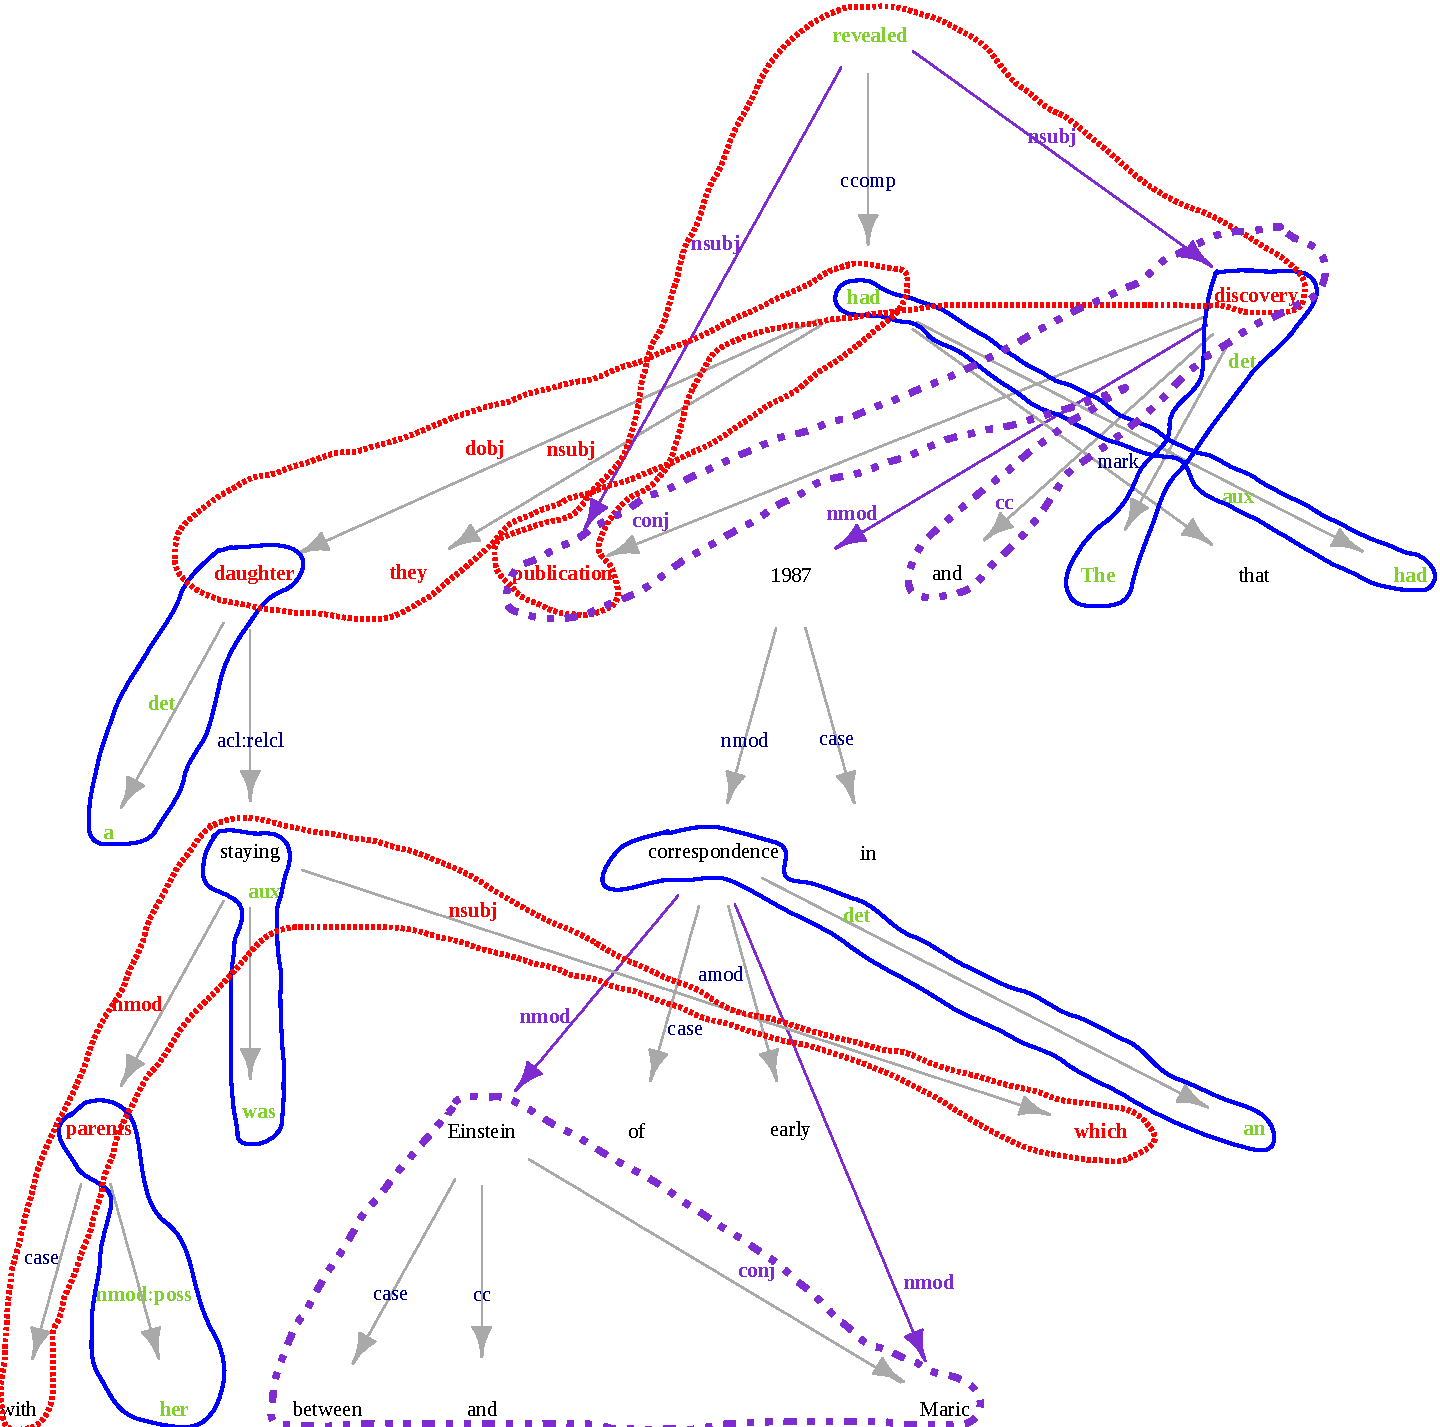
\includegraphics[width=\textwidth]{fig/05language/01DependencyGraph_match}
	\caption{Underlying which part of the dependency graph are matched by the patterns outlined in Figure \vref{fig:diagramtable}. The blue matches represent the first graph matching rule, the purple ones with the loose dashing represent the second one, while the last one with the thick dashes represent the last one.}
	\label{fig:dependencygraph_matches}
\end{figure*}


\begin{example}
Despite the possibility of performing multiple matches and rewriting as the previous examples showed, this approach is not always possible. After explicitely defining what a generalized graph grammar is, let us suppose to want to match simultaneously all the pattern graphs that were previously provided. The result of such matching phase is then depicted in Figure \ref{fig:dependencygraph_matches}: if we now compare the matches with the expected transformations, we can see that some times we would return both matched contents and aggregated ones while, on the other hand, we would like that the changes provided by one of the grammar rules are kept in the following matching phases. You can test such outcomes by using the \texttt{Sherlock} project.

In order to avoid such conflicts, the only thing that is possible to do is to subdivide one single generalized graph grammar rule into more subsequent matching and rewriting steps. The next chapter will provide an example of such operator, that will allow us to generalize the nesting for semistructured and nested relational data for graphs. 
\end{example}
